\section{Results}
We evaluated the framework on several benchmark PDEs, as summarized in Table~\ref{tab:pde-summary}. Detailed discretization schemes, solver configurations, grid coarsening procedures, and adjoint derivations are provided in Appendices~\ref{sec:AD}--\ref{sec:SWE-Tohoku}. PDE1 (Advection--Diffusion) and PDE2 (Navier--Stokes, SA model) serve as testbeds for systematic experiments, illustrating how the framework responds to varying amounts of training data and different degrees of freedom in the inputs. PDE3 (Shallow Water Equations) extends this evaluation to a large-scale application, demonstrating the framework’s scalability and robustness in complex geophysical flow settings. Sensitivity constraints were applied to multiple established operator families, including FNO, WNO, and DeepONet. Since the method aligns most naturally with FNO, we present SC-FNO results in the main text, while full comparisons with SC-WNO and SC-DeepONet, along with implementation details and theoretical analysis, are provided in the Supplementary Material. Across all PDE benchmarks, we adopted a unified experimental protocol encompassing both forward prediction and inverse inference settings, enabling evaluation of predictive accuracy as well as gradient fidelity; full experimental details are provided in Appendix~\ref{sec:EXP}. Models were trained with varying sample sizes to investigate data efficiency and to quantify the trade-off between accuracy improvements and the additional computational cost introduced by sensitivity constraints.

We also evaluated model performance under different input resolutions to assess how increasing the degrees of freedom in gridded parameter fields influences accuracy and computational cost. Both forward prediction and inversion tasks were evaluated as complementary components of the modeling framework. Forward prediction assesses each model’s ability to forecast future states from partial trajectories and parameter fields, while inversion quantifies its capacity to recover hidden input fields or governing parameters directly from observed solution states. For PDE3, corresponding to large-scale tsunami propagation governed by the Shallow Water Equations, we additionally employ a three-stage inversion framework to reconstruct the earthquake-induced Okada deformation and associated fault parameters from early tsunami gauge observations. To further assess robustness, out-of-distribution (OOD) generalization is evaluated by testing models trained on a subset of earthquake epicenter configurations against unseen cases, thereby quantifying extrapolation capability beyond the training distribution. We measure dataset preparation time, Jacobian computation time, and model training time. In the main paper, we report the total wall-clock time, which includes both CPU and GPU computing times. Detailed breakdowns for each benchmark are provided in Tables~\ref{tab:PDE1_total_computational_cost}, \ref{tab:PDE2_total_computational_cost}, and \ref{tab:PDE3_total_computational_cost} in Appendix~\ref{sec:cpu_time}, corresponding to PDE1, PDE2, and PDE3, respectively. This unified setup allows for direct comparisons of accuracy, efficiency, and robustness across PDEs.

\begin{table}[htbp]
    \centering
    \caption{\scriptsize\textbf{Summary of benchmark problems used to evaluate the performance of the Sensitivity-Constrained Neural Operator across different classes of parametric differential equations.}}
    \label{tab:pde-summary}
    \tiny
    \begin{tabular}{p{0.15\textwidth}p{0.55\textwidth}p{0.18\textwidth}}
        \hline
        Governing law & Equation form & Randomly varied input\\
        \hline
        PDE1: Advection--Diffusion &
        $\frac{\partial C}{\partial t} + \nabla \cdot \bigl( \mathbf{u}(\mathbf{x}) C \bigr) = D \nabla^2 C$ &
        $\mathbf{u}(\mathbf{x})$ and $C_0$\\[1em]
        
        PDE2: Navier--Stokes (SA Model) &
        $\nabla^2 \Psi = -\Omega$, 
        $\frac{\partial \Omega}{\partial t} 
        + \frac{\partial \Psi}{\partial x_2} \frac{\partial \Omega}{\partial x_1} 
        - \frac{\partial \Psi}{\partial x_1} \frac{\partial \Omega}{\partial x_2} 
        = \nabla \cdot \bigl[ (\nu + \nu_t) \nabla \Omega \bigr] + f(\mathbf{x}, p)$ &
        $f(\mathbf{x}, p)$ and $\Omega_0$ \\[1em]
        
        PDE3: Shallow Water Equations (SWE) &
        $\frac{\partial h}{\partial t} + \nabla \cdot (h \mathbf{u}) = 0$,
        $\frac{\partial (h \mathbf{u})}{\partial t} 
        + \nabla \cdot \bigl( h \mathbf{u} \otimes \mathbf{u} + \frac{1}{2} g h^2 I \bigr) 
        = -gh \nabla z_b + \text{Friction}$ &
        $z_b(\mathbf{x})$ and $h_0$\\
        \hline
    \end{tabular}
\end{table}


\subsection{Near-real-time Tsunami Source Inversion and Forecasting}
\label{sec:SWE-Tohoku}
\subsubsection{Real-time Tsunami Inversion Now Possible}





We demonstrate the practical consequences of this scaling regime by solving a problem previously considered infeasible: near--real-time inversion of a spatially distributed tsunami source from sparse offshore observations for the 2011 Tōhoku event (Appendix~\ref{sec:SWE-Tohoku}). Early-period buoy observations (water stage) are used to infer the tsunami deformation field and Okada parameters and to forecast subsequent evolution. The neural operators are pretrained on high-resolution, validated finite-volume simulations (Figure~\ref{fig:tohoku_validation}), with SC-NOs additionally constrained by adjoint sensitivities of the final water stage with respect to bed topography. Training simulations are generated on a high-resolution base grid ($308{,}001$ irregular mesh points) to ensure numerical accuracy, but all learning experiments use a fixed $100\times100$ grid. 

We use a three-stage inversion workflow for the real-world tsunami forecasting case, with full details provided in Appendix~\ref{sec:SWE-Tohoku}. First, a coarse seafloor deformation field is estimated by optimizing it directly through the differentiable SC-FNO surrogate using the first 30 minutes of buoy observations. The mismatch between observed and predicted water levels is computed at buoy locations, and gradients are backpropagated to update the deformation field.

Because this full-field inversion is underconstrained by sparse, short-window observations, we regularize it using a nine-parameter Okada representation. A pretrained encoder maps the Stage~1 deformation estimate to Okada parameters, and a decoder maps these parameters back to a deformation field. The parameters are then refined through the decoder and neural operator to better match the buoy observations, yielding a physically admissible source estimate for forecasting the full tsunami evolution.


\begin{figure}[ht!]
\centering
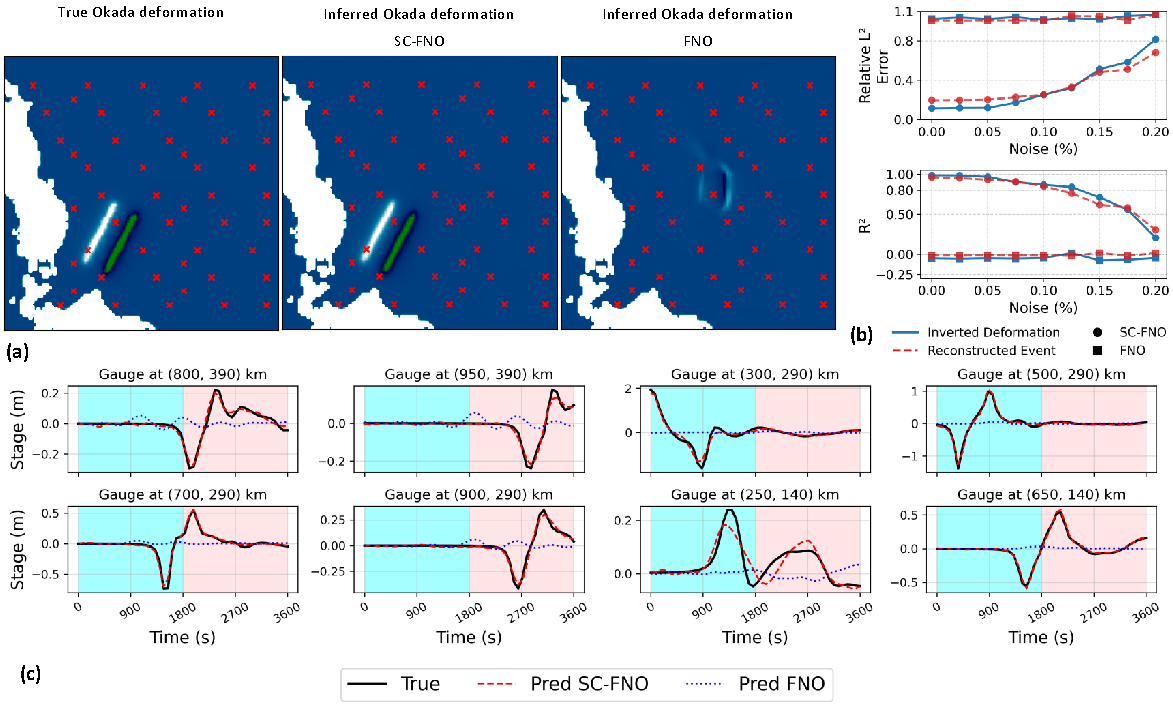
\includegraphics[width=0.9\textwidth, trim={0 0 0 0}, clip]{Figuers/PDE3_inversion_main_text_with_noise.pdf}
    \caption{\scriptsize\textbf{Multi-Stage Source Inversion and Tsunami Reconstruction.}
    (a) Visual comparison of the ground-truth Okada deformation field and the inferred deformation fields obtained from SC-FNO and FNO following Stage~3 inversion; red crosses indicate buoy locations used as observational constraints.
    (b) Comparison of Relative $L^2$ error (top) and $R^2$ score (bottom) for SC-FNO and FNO. The metrics are evaluated for both the inverted source deformation (solid lines) and the reconstructed event (dashed lines) derived from observation data with varying noise intensities.  
    (c) Representative tsunami gauge time series generated using the reconstructed deformation fields. The cyan shaded region denotes the observation window used for inversion, while the light red region indicates the extrapolation (forecasting) period. SC-FNO maintains accurate phase and amplitude tracking throughout the forecast, whereas the FNO baseline diverges significantly beyond the observation window.}
\label{fig:PDE3_inversion_main_text}
\end{figure}

This resolution balances physical fidelity with the cost of generating and storing large training sets and adjoint sensitivities and is representative of real-time warning-system practice. Although SC-NO can operate at higher resolutions, doing so substantially increases the computational cost without changing the conclusions. After completing a challenging inversion task, SC-FNO can accurately estimate deformation (Figure~\ref{fig:PDE3_inversion_main_text}a) and then forecast tsunami impacts, a feat not achievable with a conventional surrogate. Even when accounting for measurement noise, SC-FNO produces reliable inversions up to $\sim10\%$ noise (Figure~\ref{fig:PDE3_inversion_main_text}b). 

Time series at multiple gauges show that the timing, wave heights, negative leading waves, and positive trailing waves are all reproduced well by SC-FNO across minor ($<0.3$ m), advisory-level (0.3--1.0 m), and significant ($>1$ m) impact ranges, both within and beyond the observation window (Figure~\ref{fig:PDE3_inversion_main_text}c). In contrast, the standard FNO completely fails to recover a meaningful deformation field (Figure~\ref{fig:PDE3_inversion_main_text}a) and produces inaccurate forecasts (Figure~\ref{fig:PDE3_inversion_main_text}c). Overall, SC-FNO achieves more than an order-of-magnitude reduction in relative $L^2$ error and near-perfect $R^2$ scores for both the inverted deformation and the reconstructed tsunami event, with additional results shown in Figures~\ref{fig:stage1_field_inversion}, \ref{fig:stage3_param_inversion}, and~\ref{fig:gauge_timeseries}. Remarkably, the full three-stage inversion and forward reconstruction, involving thousands of high-resolution surrogate evaluations, takes only 4.5 minutes on a single NVIDIA A100 GPU, clawing back precious time for possible real-time warnings. As discussed earlier, most current warning systems rely on precomputed datasets, which struggle to resolve the impacts of diverse deformation fields \citep{titov2005real, ishiwatari2012tsunami}. Our workflow provides a foundation for tiered, real-time, full-fidelity warning systems with substantially improved accuracy. It also uses a physically aligned upscaling procedure to recover fine-scale fields from coarse predictions while ensuring consistency with the coarse mean depth and incorporating bed topography (Figure~\ref{fig:upsampling_comparison}).

\subsubsection{Accurately Capturing Shocks Caused by (Gridded) Seafloor Deformation:}
We consider a more idealized experiment in which neural operators pretrained on $1{,}000$ training samples are evaluated solely on their forward-run quality with precise deformation inputs, thus ignoring discrepancies in their inversion capabilities. SC-FNO remains closely aligned with the ground truth across time snapshots (Figure~\ref{fig:PDE3_All}a), whereas the FNO exhibits significant dissipative drift and structural loss. Although the FNO visually produces passable wave propagation, it misrepresents the timing of the first peak and the height of secondary impacts (Figure~\ref{fig:PDE3_All}d--e) and incurs a much faster accumulation of error (Figure~\ref{fig:PDE3_All}f). When examining a metric of real-world importance, the FNO exhibits an almost three-times higher false negative rate (16.7\%) compared to SC-FNO (5.9\%), suggesting substantially different warning outcomes.

\begin{figure}[ht!]
    \centering
    
\includegraphics[width=0.98\textwidth, trim={0 0 0 0}, clip]{Figuers/PDE3_All.pdf} % Replace with the actual filename if different
        
    \caption{\scriptsize\textbf{Shallow Water Equations (PDE3) for Tsunami Propagation and Inundation.}  
    (a) A sample tsunami event (epicenter location and deformation) showing the ground truth, along with the forward predictions of SC-FNO and FNO. Both models were trained using 1000 samples.   (b) In-training computing cost vs.\ error.  
    (c) Out-of-training-distribution (OOD) computing cost vs.\ error.  
    (d) Time series of water stage at a representative point.  
    (e) Absolute error at the same point.  
    (f) Cumulative relative $L^2$ error over time.  
    (g) Forward prediction errors at 1000 in-training and OOD samples.  
    (h) Inundation extent classification accuracy for in-training and OOD samples.}  

    \label{fig:PDE3_All}
\end{figure}



\subsubsection{Generalizing Out-of-Distribution (OOD):}

The contrasts between SC-FNO and FNO become even more pronounced for spatially OOD events, rendering the conventional surrogate ineffective. In this benchmark, OOD refers to tsunami events whose earthquake epicenters are \emph{disjoint} from the region used during training, with some points located more than 150\,km away from the nearest training sample (Supplementary Figure~\ref{fig:nse_sampling_strategies}). The false negative ratio of the FNO is 2.8 times that of SC-FNO in the training region, while it increases to 3.6 times in the OOD region (Figure~\ref{fig:PDE3_All}g). SC-FNO maintains approximately $\sim88\%$ accuracy for OOD events, whereas the FNO drops precipitously to $55\%$, making it unusable for all practical purposes (Figure~\ref{fig:PDE3_All}h). This experiment illustrates OOD behavior clearly in space, but OOD also commonly arises in parameter space and can be difficult to detect during real-world use. OOD reliability is critical to support inversion.

\subsection{Systematic Explanatory Scaling Benchmarks}
\label{sec:AD_NSE}
The tsunami inversion problem entangles discretization, dimensionality, nonlinearity, and inverse conditioning. To isolate these effects, we design systematic scaling benchmarks using advection--dispersion (ADE) and Reynolds-averaged Navier--Stokes (RANS) equations (Appendices~\ref{sec:AD}--\ref{sec:NSE-SA}), which provide smooth, controlled testbeds. For ADE, the models forecast the concentration field from early snapshots and velocity inputs, whereas for RANS they autoregressively predict vorticity evolution given the initial vorticity and distributed forcing.

\subsubsection{The Curse of Dimensionality, Reversed:}
Standard empirical learning relies on observing outcomes across parameter combinations, whereas sensitivity-constrained training augments each sample with gradient information with respect to all input parameters, obtained efficiently via backpropagation \citep{rumelhart1986learning}. This additional information per sample underlies the scaling behavior examined next. Here, to isolate the effect of input dimensionality, we run training experiments for RANS that vary only the intrinsic resolution of the initial conditions (DOF $=4^2$, $16^2$, $64^2$), upsample the fields to the same base grid resolution used in training ($64\times64$), and hold all other factors constant (Appendix~\ref{sec:AD_NSE}, Section~\textit{Degree of freedom (DOF) experiment}). The neural operators are trained with varying numbers of samples; smooth curves are then fitted to the error--cost points for each method, allowing us to read off the computational cost required to reach specific error levels.




% New Merged Figure for PDE1
\begin{figure}[ht!]
    \centering
    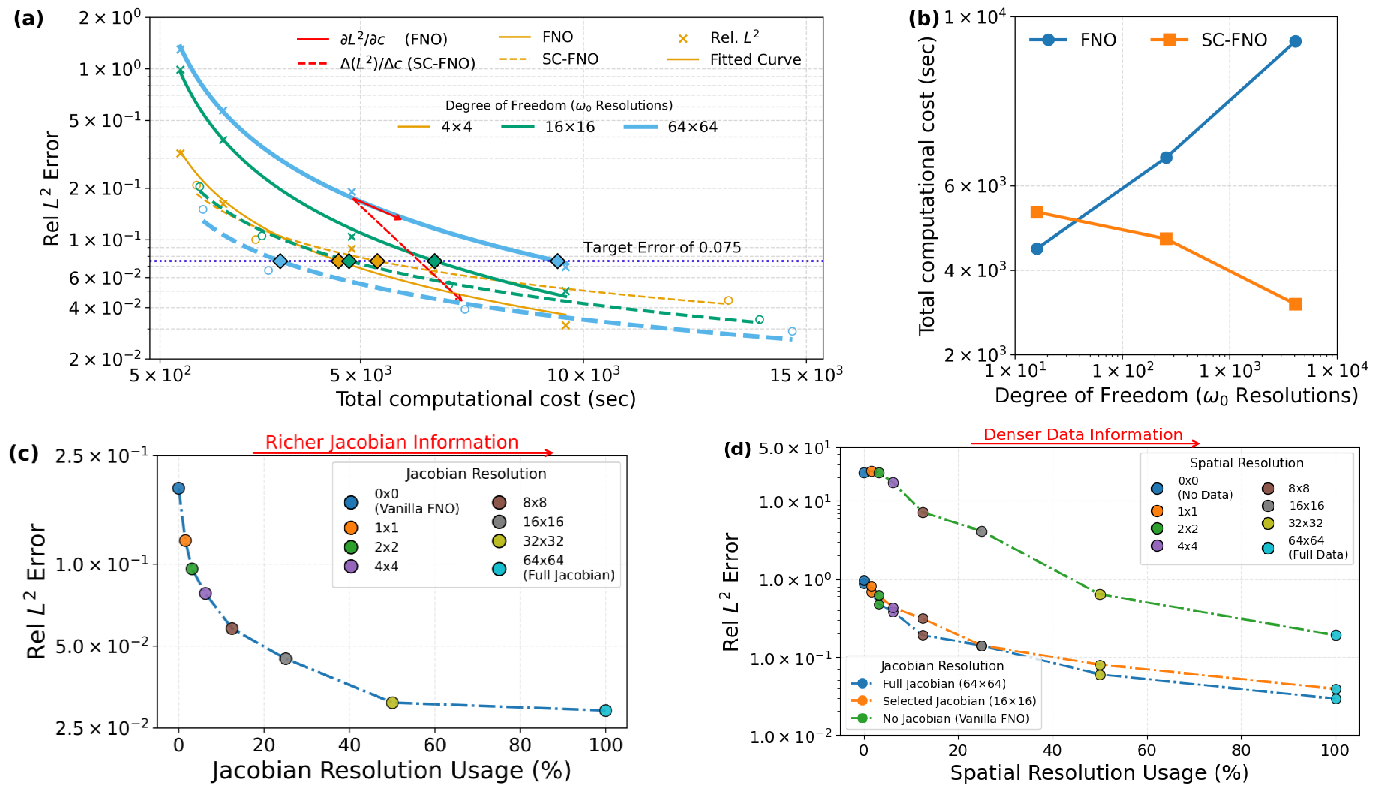
\includegraphics[width=0.98\textwidth, trim={0 0 0 0}, clip]{Figuers/scaling curve.pdf}
    
    \caption{\scriptsize
    Computational efficiency and information scaling of NOs.
    \textbf{(a)} Relative $L^2$ error versus total computational cost (including data generation and training) for increasing degrees of freedom in the input field $\omega_0$. Curves correspond to different intrinsic parameter degree of freedom (DOF), illustrating the trade-off between accuracy and cost for FNO and SC-FNO.
    \textbf{(b)} Total computational cost required to reach a target relative $L^2$ error of $0.075$ as a function of $\omega_0$ degrees of freedom. These values are obtained by intersecting the horizontal error threshold with the curves in panel (a). The red solid arrow indicates the error reduction rate per unit computational cost achieved by increasing training samples for FNO, while the red dashed arrow connects FNO and SC-FNO at fixed resolution and sample count. Its slope, $\Delta(L^2)/\Delta(c)$ (SC-FNO), quantifies the substantially steeper error reduction obtained by incorporating sensitivity constraints compared to data-only scaling, $\partial L^2/\partial c$ (FNO).
    \textbf{(c)} Sensitivity of model accuracy to Jacobian supervision density. Using the solution on a $64\times64$ grid at the final time step for gradient computation, subsets of the full Jacobian $[64\times64,\,64\times64]$ are progressively included in the loss. Increasing Jacobian resolution yields monotonic error reduction, demonstrating the benefit of richer sensitivity information.
    \textbf{(d)} Sensitivity of performance to spatial data resolution under full, partial, and no Jacobian supervision. For a fixed computational budget, SC-FNO achieves lower error across resolutions, highlighting the complementary roles of state data and gradient information in improving operator learning efficiency.
    }
    
    
    \label{fig:scaling_curve}
\end{figure}


While increasing the input DOF leads to elevated errors for the standard FNO, as expected, a surprising reverse scaling pattern emerges for SC-FNO. Specifically, increasing the DOF from $4^2$ to $64^2$ produces progressively larger uncertainty and relative $L^2$ errors for the FNO, or a higher computational cost to achieve the same accuracy (Figure~\ref{fig:scaling_curve}a). Accordingly, to maintain the error fixed at $0.075$, the total compute cost for the FNO grows from roughly $4000$\,s to $9600$\,s (Figure~\ref{fig:scaling_curve}b), driven primarily by the need for larger training datasets. In contrast, sensitivity-constrained models exhibit a monotonic reduction in error with increasing input dimensionality, a reversal of the canonical behavior. For the same accuracy threshold, the estimated compute cost for SC-FNO even slightly decreases from approximately $2000$\,s to $1900$\,s—both far smaller than the cost required by the FNO. To our knowledge, such reverse scaling has not been previously reported for data-driven learning. We further conducted an ablation study in which the fraction of the Jacobian used during training was systematically varied. We observed a steep early reduction in error as a large fraction of the Jacobian is used (Figure~\ref{fig:scaling_curve}c, initially sharper than the impact of data in Figure~\ref{fig:scaling_curve}d), followed by gradual saturation beyond approximately $50\%$. This behavior is directly linked to the observed reverse scaling curve.

Several reasons explain this favorable scaling behavior. First, sensitivity-constrained training is notably more cost-effective than generating computational data, especially in the low-data regime, as shown by the arrow-annotated slopes ($\mathrm{d}L^2/\mathrm{d}(\text{cost})$). Second, the effects of Jacobian supervision are significant—quickly reducing errors by roughly a factor of three to ten—and size-dependent, as it takes a large portion of the Jacobian to reach information saturation. A larger supervised Jacobian matrix more effectively suppresses uncertainty. Lastly, and most importantly, the size of the Jacobian is large ($64^2 \times \text{DOF}$, where DOF is specified above, even when considering only the solution at the final time step) compared to the numerical solution ($64^2 \times 50$), and it scales with DOF, thereby constraining many directions of the model at modest cost. This increase in supervisory power effectively counters, and in this case even outweighs, the increase in uncertainty. As a result, either the same computational cost leads to reduced error, or a smaller training sample is required to achieve a fixed accuracy. Stated another way, sensitivity supervision effectively neutralizes (``hedges against'') the combinatorial growth of uncertainty associated with high-dimensional inputs, so that the number of training samples no longer needs to increase when moving from a dozen parameters to full two-dimensional or three-dimensional input representations. We note that a higher DOF often increases base computational costs, but our design here isolates the effects of DOF.




% New Merged Figure for PDE1
\begin{figure}[ht!]
    \centering
    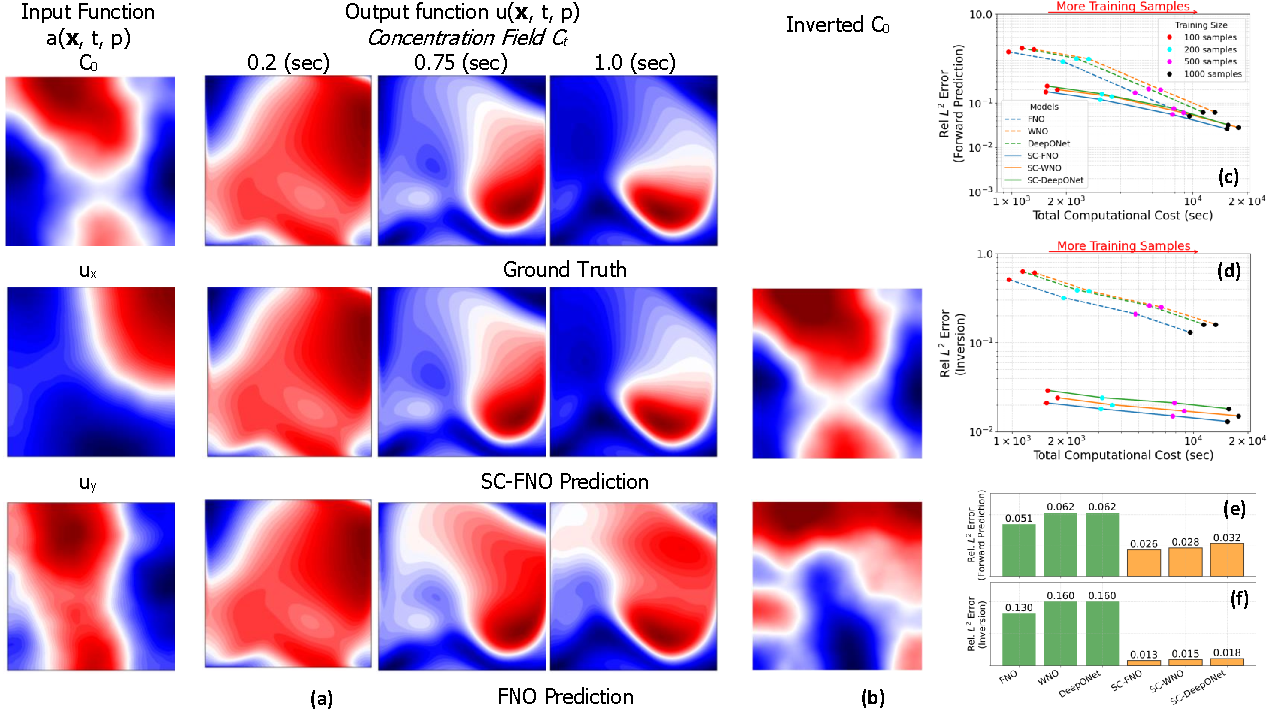
\includegraphics[width=0.98\textwidth, trim={0 0 0 0}, clip]{Figuers/PDE1_sample_prediction_Errors.pdf}
    \caption{\scriptsize
    Representative forward prediction, inversion, and accuracy--computation trade--off for the advection--diffusion problem with spatially varying velocity and initial concentration (PDE1).
    \textbf{(a)} Sample forward prediction showing the input initial concentration field $C_0$, velocity components $(u_x,u_y)$, and solution snapshots $u(x,t)$ at selected times. Ground truth, SC-FNO prediction, and FNO prediction values are shown for comparison.
    \textbf{(b)} Inversion results for the initial concentration field $C_0$, reconstructed from solution observations using models trained with 200 samples.
    \textbf{(c)} Relative $L^2$ error for forward prediction versus total computational cost as the number of training samples increases.
    \textbf{(d)} Relative $L^2$ error for inversion (reconstruction of $C_0$) versus total computational cost.
    \textbf{(e)} Relative $L^2$ error for forward prediction at 1000 training samples.
    \textbf{(f)} Relative $L^2$ error for inversion at 1000 training samples.
    Across all settings, sensitivity-constrained models consistently achieve lower errors than their unconstrained counterparts for the same computational budget.
    }
        
    \label{fig:PDE1_summerised_merged}
\end{figure}



\subsubsection{Jacobian Resolves Discretization-Induced Ill-Posedness for Surrogates:}
Equipped with the scaling theory above and aiming to explain why SC-FNO can uniquely handle varying deformation fields in the tsunami case, we conduct a series of systematic experiments in which both initial conditions and forcing parameters (concentration in ADE and vorticity in RANS) are randomly sampled from Gaussian random fields (details are provided in Appendix~\ref{sec:EXP}).

With such randomly varying gridded parameters, conventional surrogate models rapidly lose reliability, even at moderate data scales. In ADE, the standard FNO exhibits excessive numerical diffusion and progressive smoothing of advected concentration fronts, whereas SC-FNO preserves sharp transport features at a comparable training cost (Supplementary Figure~\ref{fig:PDE1_sample_pred}). In RANS, reducing the training set to 500 samples causes the standard FNO to distort vortex shapes and smear vortical channels, accompanied by a loss of boundary sharpness, while SC-FNO maintains coherent vortical structures over the same time horizon at a comparable cost (Supplementary Figure~\ref{fig:PDE2_sample_pred}).

These issues are all reflections of the high-dimensionality challenge—the standard FNO can eventually achieve acceptable accuracy when there is a large training set ($\sim$1000 samples), whereas SC-FNO remains well behaved with as few as 200 samples (Figures~\ref{fig:PDE1_summerised_merged}a and Supplementary ~\ref{fig:PDE2_summerised}a) due to the scaling property discussed above. Achieving a relative error of $1\times10^{-1}$ requires roughly four times more data for the FNO than for SC-FNO. Similar trends are observed for WNO and DeepONet, indicating a generic limitation of conventional operator training. Consistent with the experiments above, SC-NOs remove large errors rapidly in the low-data regime but exhibit slower asymptotic error decay in the higher-data regime, consistent with information saturation from Jacobian supervision and a deliberate trade-off between pointwise accuracy and sensitivity fidelity.

Many surrogate models fail for high-dimensional problems because they cannot resolve how solutions vary with thousands of inputs, forcing retraining for each new field. For example, flood-inundation surrogates often fail to represent detailed topographic effects, requiring them to be trained separately for each domain \citep{zanchetta2022probabilistic}. Turbulence models struggle to generalize across geometries and flow conditions \citep{duraisamy2019turbulence}, and cardiac biomechanics surrogates lose essential structures across spatially varying material fields \citep{cai2021surrogate}. SC-NOs offer a potential solution to this long-standing challenge at operationally relevant scales.




\subsubsection{Restoring Tractability in Parameter--Function Inversion:}
Here, we show that the difficulty of standard neural operator inversion can be attributed to unfavorable scaling behavior, while SC-NOs address this challenge, which is impractical to overcome through brute-force data collection. To remove data limitations as a confounding factor, we recover the underlying input fields (the initial concentration field $C_0(\mathbf{x})$ for ADE and the vorticity field $\omega_0(\mathbf{x})$ for RANS) using gradient descent, pretrained neural operators, and full-domain data (rather than sparse data, as in the tsunami case).

We observe slowly descending inversion error--cost scaling curves, with performance gaps between standard NOs and SC-NOs far exceeding those observed in the forward setting (Figures~\ref{fig:PDE1_summerised_merged}b and Supplementary ~\ref{fig:PDE2_summerised}b). Extrapolating these lines suggests that ordinary NOs would require two to three orders of magnitude more training data—which is economically unjustifiable, if not impossible—to approach the inversion accuracy of SC-NOs. Consequently, representative inversion examples (Supplementary Figure~\ref{fig:PDE1_C0_inversion} for ADE and Figure~\ref{fig:PDE2_w0_inversion} for RANS) show that SC-FNO, SC-WNO, and SC-DeepONet accurately reconstruct the underlying fields, while their unconstrained counterparts recover solutions bearing little resemblance to the ground truth. These results further suggest that standard NOs can produce passable forward solutions while encoding entirely incorrect internal relationships.

During gradient-based inversion, the surrogate is repeatedly evaluated at unseen inputs, pushing it outside the training distribution. Models without sensitivity constraints respond unpredictably under such conditions, often steering optimization toward non-physical solutions. If a gradient-free, response-surface-type inversion algorithm were used instead, it would be unlikely to scale to the dimensionality required to estimate high-dimensional inputs. While the inversion advantage of SC-FNO was demonstrated previously \citep{behroozi2025sensitivity}, here this advantage persists for unprecedentedly high-dimensional gridded inputs. The drastically improved scaling curves of SC-NOs, as discussed above, make practically important inversion cases (as shown in the tsunami case) tractable. Many applications require forcing and flow conditions to be inferred from sparse or indirect observations before making predictions.


\subsubsection{Stabilizing Long-Horizon Rollout Through Sensitivity Constraints:}
Temporal rollout remains a major challenge for AI-based PDE solvers, as small one-step errors can accumulate into rapid divergence under autoregressive prediction. To evaluate this effect, we use RANS in a recurrent one-step rollout setting, training models to predict the next state from the current state and then applying the learned transition operator autoregressively for long-horizon forecasts.

The FNO suffers substantial error accumulation during rollout, whereas SC-FNO maintains functional predictions with much lower error (Figure~\ref{fig:PDE2_rollout}a--b). SC-FNO tracks the true vorticity evolution with accurate phase and amplitude far beyond the training horizon, whereas the FNO exhibits progressive phase drift and amplitude errors. Although neither scheme can fully prevent errors from accumulating, Figure~\ref{fig:PDE2_rollout}c shows that SC reduces rollout errors by $\sim3\times$. The improved temporal stability of SC-FNO arises from its explicit control of integrated sensitivities, which reduce error amplification along unstable directions of the system’s dynamics—modes that strongly amplify small perturbations and are a common source of phase drift and dissipation. In contrast, standard FNOs minimize only pointwise prediction error, allowing small gradient mismatches to accumulate under autoregressive rollout. The sensitivity constraint therefore acts as a structural regularizer that preserves the correct linearized dynamics, yielding a more stable transition operator and slower error growth over long horizons.

% \subsubsection{Limitations:}


\begin{figure}[htbp]
    \centering
    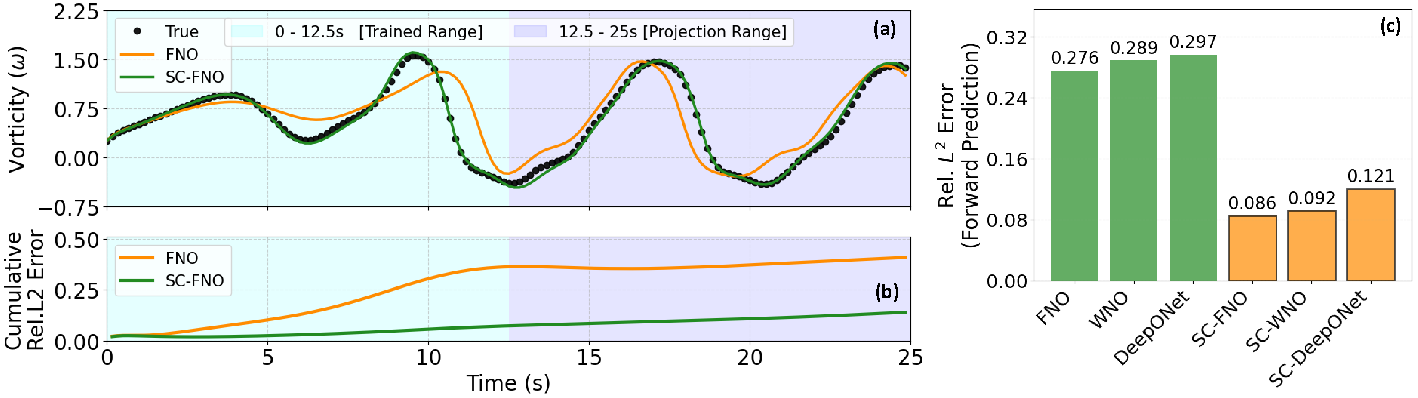
\includegraphics[width=0.98\textwidth, trim={0 0 0 0}, clip]{Figuers/NSE_time_serie.pdf}
    \caption{\scriptsize\textbf{Rollout forecasting (PDE2).}  
    (a) Vorticity time series showing SC-FNO closely matches ground truth beyond the training horizon.  
    (b) Cumulative relative $L^2$ error highlighting reduced error growth with SC-FNO.  
    (c) Rollout errors comparing FNO and SC-FNO models trained with 1000 samples.}              
    \label{fig:PDE2_rollout}
\end{figure}


















